
\chapter{Appendix}



\section{Somato-dendritic coupling}\label{sec-somato-dendr}

\cite{urbanczik2014learning} discuss a possible extension to their neuron- and plasticity model, in which the
dendro-somatic coupling transmits voltages in both directions. They show that the plasticity rule requires only minor
adaptations for successful learning under this paradigm. Yet, as described by passive cable theory, the flow between
neuronal compartments is dictated by their respective membrane capacitances. These are calculated from their membrane
areas, which vastly differ in the case of pyramidal neurons. \todo{find a nice citation for this}


15,006 458


will not be considered here. The motivation is, that dendritic membrane area is


\section{Integration of the spike-based Urbanczik-Senn plasticity}



Starting with the complete Integral from $t=0$.

\begin{align}
  \Delta W_{ij}(0,t) & =\eta \int_0^t dt' \  \int_0^{t'} dt'' \ \kappa(t'-t'') V_i^\ast (t'') s_j^\ast (t'')                          \\
                     & = \eta \int_0^t dt'' \  \int_{t''}^{t} dt' \ \kappa(t'-t'') V_i^\ast (t'') s_j^\ast (t'')                      \\
                     & = \eta \int_0^t dt'' \  \left[ \tilde{\kappa}(t-t'') - \tilde{\kappa}(0) \right] V_i^\ast (t'') s_j^\ast (t'') \\
\end{align}

With $\tilde{\kappa}$ being the antiderivative of $\kappa$:

\begin{align}
  \kappa(t)         & = \frac{\delta}{\delta t} \tilde{\kappa}(t) \\
  \tilde{\kappa}(t) & = - e^{-\frac{t}{t_{\kappa}}}               \\
\end{align}

The above can be split up into two separate integrals:

Which implies the identities

\begin{align}
  I_1(t_1, t_2 + \Delta t) & = I_1 (t_1, t_2) + I_1 (t_2, t_2 + \Delta t)                                       \\
  I_2(t_1, t_2 + \Delta t) & = e^{- \frac{t_2 - t_1}{\tau_{\kappa}}} I_2 (t_1, t_2) + I_2 (t_2, t_2 + \Delta t)
\end{align}


\begin{align}
  I_2 (t_1, t_2 + \Delta t) & = -\int_{t_1}^{t_2 + \Delta t} dt' \ \tilde{\kappa} (t_2 + \Delta t - t') V_i^\ast (t') s_j^\ast (t')                                        \\
                            & = -\int_{t_1}^{t_2} dt' \ \left[ -e^{- \frac{t_2 + \Delta t - t'}{\tau_\kappa}} \right] V_i^\ast (t') s_j^\ast (t')
  -\int_{t_2}^{t_2 + \Delta t} dt' \ \left[ -e^{- \frac{t_2 + \Delta t - t'}{\tau_\kappa}} \right] V_i^\ast (t') s_j^\ast (t')                                             \\
                            & = -e^{- \frac{ \Delta t}{\tau_\kappa}} \int_{t_1}^{t_2} dt' \ \left[ -e^{- \frac{t_2 - t'}{\tau_\kappa}} \right] V_i^\ast (t') s_j^\ast (t')
  -\int_{t_2}^{t_2 + \Delta t} dt' \ \left[ -e^{- \frac{t_2 + \Delta t - t'}{\tau_\kappa}} \right] V_i^\ast (t') s_j^\ast (t')
\end{align}


Using this we can rewrite the weight change from $t$ to $T$ as:


\begin{align}
  \Delta W_{ij}(t,T) & = \Delta W_{ij}(0,T) - \Delta W_{ij}(0,t)                                               \\
                     & = \eta [-I_2(0,T) + I_1(0,T) + I_2(0,t) - I_1(0,t)]                                     \\
                     & = \eta [I_1(t,T) - I_2(t,T) + I_2(0,t)\left( 1 - e^{- \frac{T-t}{\tau_\kappa}} \right)]
\end{align}

The simplified \cite{sacramento2018dendritic} case would be:

\begin{align}
  \frac{dW_{ij}}{dt} & = \eta (\phi(u_i) - \phi(\hat{v_i})) \phi(u_j)                                         \\
  \Delta W_{ij}(t,T) & = \int_t^T dt' \ \eta \  (\phi(u_i^{t'}) - \phi(\widehat{v_i^{t'}})) \  \phi(u_j^{t'}) \\
  \Delta W_{ij}(t,T) & = \eta \int_t^T dt' \  (\phi(u_i^{t'}) - \phi(\widehat{v_i^{t'}})) \ \phi(u_j^{t'})    \\
  V_i^*              & = \phi(u_i^{t'}) - \phi(\widehat{v_i^{t'}})                                            \\
  s_j^*              & = \kappa_s * s_j
\end{align}


Where $s_i$ is the postsynaptic spiketrain and $V_i^*$ is the error between dendritic prediction and somatic rate and
$h( u )$. The additional nonlinearity $h( u ) = \frac{d}{du} ln \  \phi(u)$ is ommited in our model \todo{should it
  though?}.




Antiderivatives:

\begin{align}
  \int_{-\infty}^x H(t)dt = tH(t) = max(0,t)
\end{align}


\begin{align}
  \tau_l & = \frac{C_m}{g_L} = 10 \\
  \tau_s & = 3
\end{align}

Writing membrane potential to history (happens at every update step of the postsynaptic neuron):

\begin{lstlisting}[language=C++, directivestyle={\color{black}}
                   emph={int,char,double,float,unsigned,exp},
                   emphstyle={\color{blue}}]

UrbanczikArchivingNode< urbanczik_parameters >::write_urbanczik_history(Time t, double V_W, int n_spikes, int comp)
{
	double V_W_star = ( ( E_L * g_L + V_W * g_D ) / ( g_D + g_L ) );
	double dPI = ( n_spikes - phi( V_W_star ) * Time::get_resolution().get_ms() )
      * h( V_W_star );
}\end{lstlisting}

I interpret this as:


\begin{align}
  \int_{t_{ls}}^T dt' \ V_i^* & = \int_{t_{ls}}^T dt' \  (s_i - \phi(V_i )) h(V_i),               \\
  \int_{t_{ls}}^T dt' \ V_i^* & = \sum_{t=t_{ls}}^T \  (s_i(t) -  \phi(V_i^t ) \Delta t) h(V_i^t) \\
\end{align}

\begin{lstlisting}[language=C++, directivestyle={\color{black}}
                   emph={int,char,double,float,unsigned,exp},
                   emphstyle={\color{blue}}]
for (t = t_ls; t< T; t = t + delta_t)
{
   	minus_delta_t = t_ls - t;
    minus_t_down = t - T;
    PI = ( kappa_l * exp( minus_delta_t / tau_L ) - kappa_s * exp( minus_delta_t / tau_s ) ) * V_star(t);
    PI_integral_ += PI;
    dPI_exp_integral += exp( minus_t_down / tau_Delta_ ) * PI;
}  
// I_2 (t,T) = I_2(0,t) * exp(-(T-t)/tau) + I_2(t,T)
PI_exp_integral_ = (exp((t_ls-T)/tau_Delta_) * PI_exp_integral_ + dPI_exp_integral);
W_ji = PI_integral_ - PI_exp_integral_;
W_ji = init_weight_ + W_ji * 15.0 * C_m * tau_s * eta_ / ( g_L * ( tau_L - tau_s ) );    
  
kappa_l = kappa_l * exp((t_ls - T)/tau_L) + 1.0;
kappa_s = kappa_s * exp((t_ls - T)/tau_s) + 1.0;
  \end{lstlisting}


\begin{align}
  \int_{t_{ls}}^T dt' s_j^* & =  \tilde{\kappa_L}(t') * s_j -  \tilde{\kappa_s}(t') * s_j
\end{align}

$I_1$ in the code is computed as a sum:

\begin{align}
  I_1 (t,T) = \sum_{t'=t}^T \ (s_L^*(t') - s_s^*(t')) * V^*(t')
\end{align}



\section{Dendritic leakage conductance}\label{sec-gl-dend}

In order to match neuron dynamics between the rate and spiking neuron implementations as closely as possible, a suitable
leakage conductance for dendritic compartments was required. For simplicity, we now consider a single synaptic
connection from neuron $i$ to neuron $j$ with weight $W_{ji}$ and attempt to identify an appropriate parameter. As
described in Equation \ref{eq-spiking-basal-compartment}, a dendritic compartment evolves according to: \todo{expand to
    multiple presynaptic neurons?}

\begin{align}
    C_m^{dend} \dot{v}_j^{dend} & = -g_l^{dend} \  v_j^{dend} +  W_{ji} \    \langle \textit{n}_i \rangle
\end{align}

Under the assumption that the activation of neuron $i$ remains static over time, we can replace the spontaneous
activation $s_i(t)$ with the expected number of spikes per simulation step $\langle \textit{n}_i \rangle = r_i \ \Delta
    t$. Next, in order to find the convergence point of the ODE, we set the left side of the equation to $0$ and attempt to
solve it:

\begin{align}
    0                        & = -g_l^{dend} \  v_j^{dend} + W_{ji} \    r_i \ \Delta t \\
    g_l^{dend} \  v_j^{dend} & = W_{ji} \    r_i \ \Delta t
\end{align}

The desired effect of presynaptic activation on the postsynaptic dendritic potential is described in Equation
\ref{eq-v-bas-rate} ($v_j^{dend} = W_{ji} \    r_i$), which occurs on both sides of the above equation. Assuming the
desired equalitiy, both terms to drop out from the equation. Thus, the correct parametrization for the dendritic leakage
conductance is:
\begin{align}
    g_l^{dend} & = \Delta t
\end{align}

It was shown experimentally, that for hight spike frequencies, this parameterization leads to an exact match of
dendritic potentials between neuron models. This value for the dendritic leakage conductance will be assumed to be the
default throughout all experiments where spiking neurons are used. \newline

In order to keep the NEST models as similar as possible, rate neurons evolve according to the same dynamics, with the
difference that they transmit their activation at every timestep. Like the original implementation, dendrites of rate
neurons do not evolve gradually, but are fully defined by presynaptic at time $t$ \footnote{Due to the synaptic delay
    enforced by the architecture of NEST, this is not entirely correct. Dendritic potentials at time $t$ are computed from
    presynaptic activity at time $t- \Delta t$, i.e. the previous simulation step.}. This behaviour is acheived by setting
the leakage conductance to $1$ for all dendritic compartments. During network initialization, dendritic leakage
conductances are set to either one of these values depending on the type of network to be trained.


\section{Plasticity in feedback connections}\label{sec-feedback-plast}

In the model by \cite{sacramento2018dendritic}, Pyramidal-to-pyramidal feedback weights evolve according to: 

\begin{align}
    \dot{w}_{l}^{down} & = \eta_l^{down} \ ( \phi(u_l^{P}) - \phi(w_l^{down} r_{l+1}^P) )\ \phi(u_{l+1}^{P})^T
\end{align}

The error term in this case on first sight differs greatly from the original Urbanczik-Senn plasticity rule. Yet it 
serves a purpose for learning and could arguably be implemented by biological neurons. An intuitive way to interpret the error
term is as the difference between somatic activity and the apical activity that can be traced back to superficial 
pyramidal neurons. In a biological neuron, this second part could plausibly be encoded by the voltage of a distal
apical compartment which is innervated only by top-down connections and leaks into the proximal apical compartment
($v^{api}$) with a conductance of $1$. The separation of pyramidal neuron apical dendrites into a proximal and a distal
tree is well documented \citeme. A difference between plasticity mechanisms for synapses arriving at these two 
integration zones is plausible, although I was unable to find prior research supporting this type of plasticity \citeme.
\newline

In the NEST implementation, the neuron model contains a distal apical compartment which is innervated exclusively by top-down
feedback connections. For simplicity, this compartment has no complex connection to the other compartments. Instead,
all events sent to it are duplicated and sent to the proximal apical compartment as well. This allows for convenient 
readout of the aforementioned error term for plasticity without affecting the neuron dynamics for simualtions where 
this compartment serves no purpose. A more sophisticated model of the apical tree which resembles pyramidal neurons more
closely could be a desirable extension to this network.

\section{Presentation times and Latent Equilibrium}\label{sec-appendix-t-pres}

Exactly matching parameters and the training environment to those of existing implementations turned out to be a
significant challenge. Particularly the way NEST handles signal transmissions made and exact numerical replication of
results impossible, as discussed in Section \todo{talk about timing differences}. In order to validate, that



\begin{figure}[t]
    \centering
    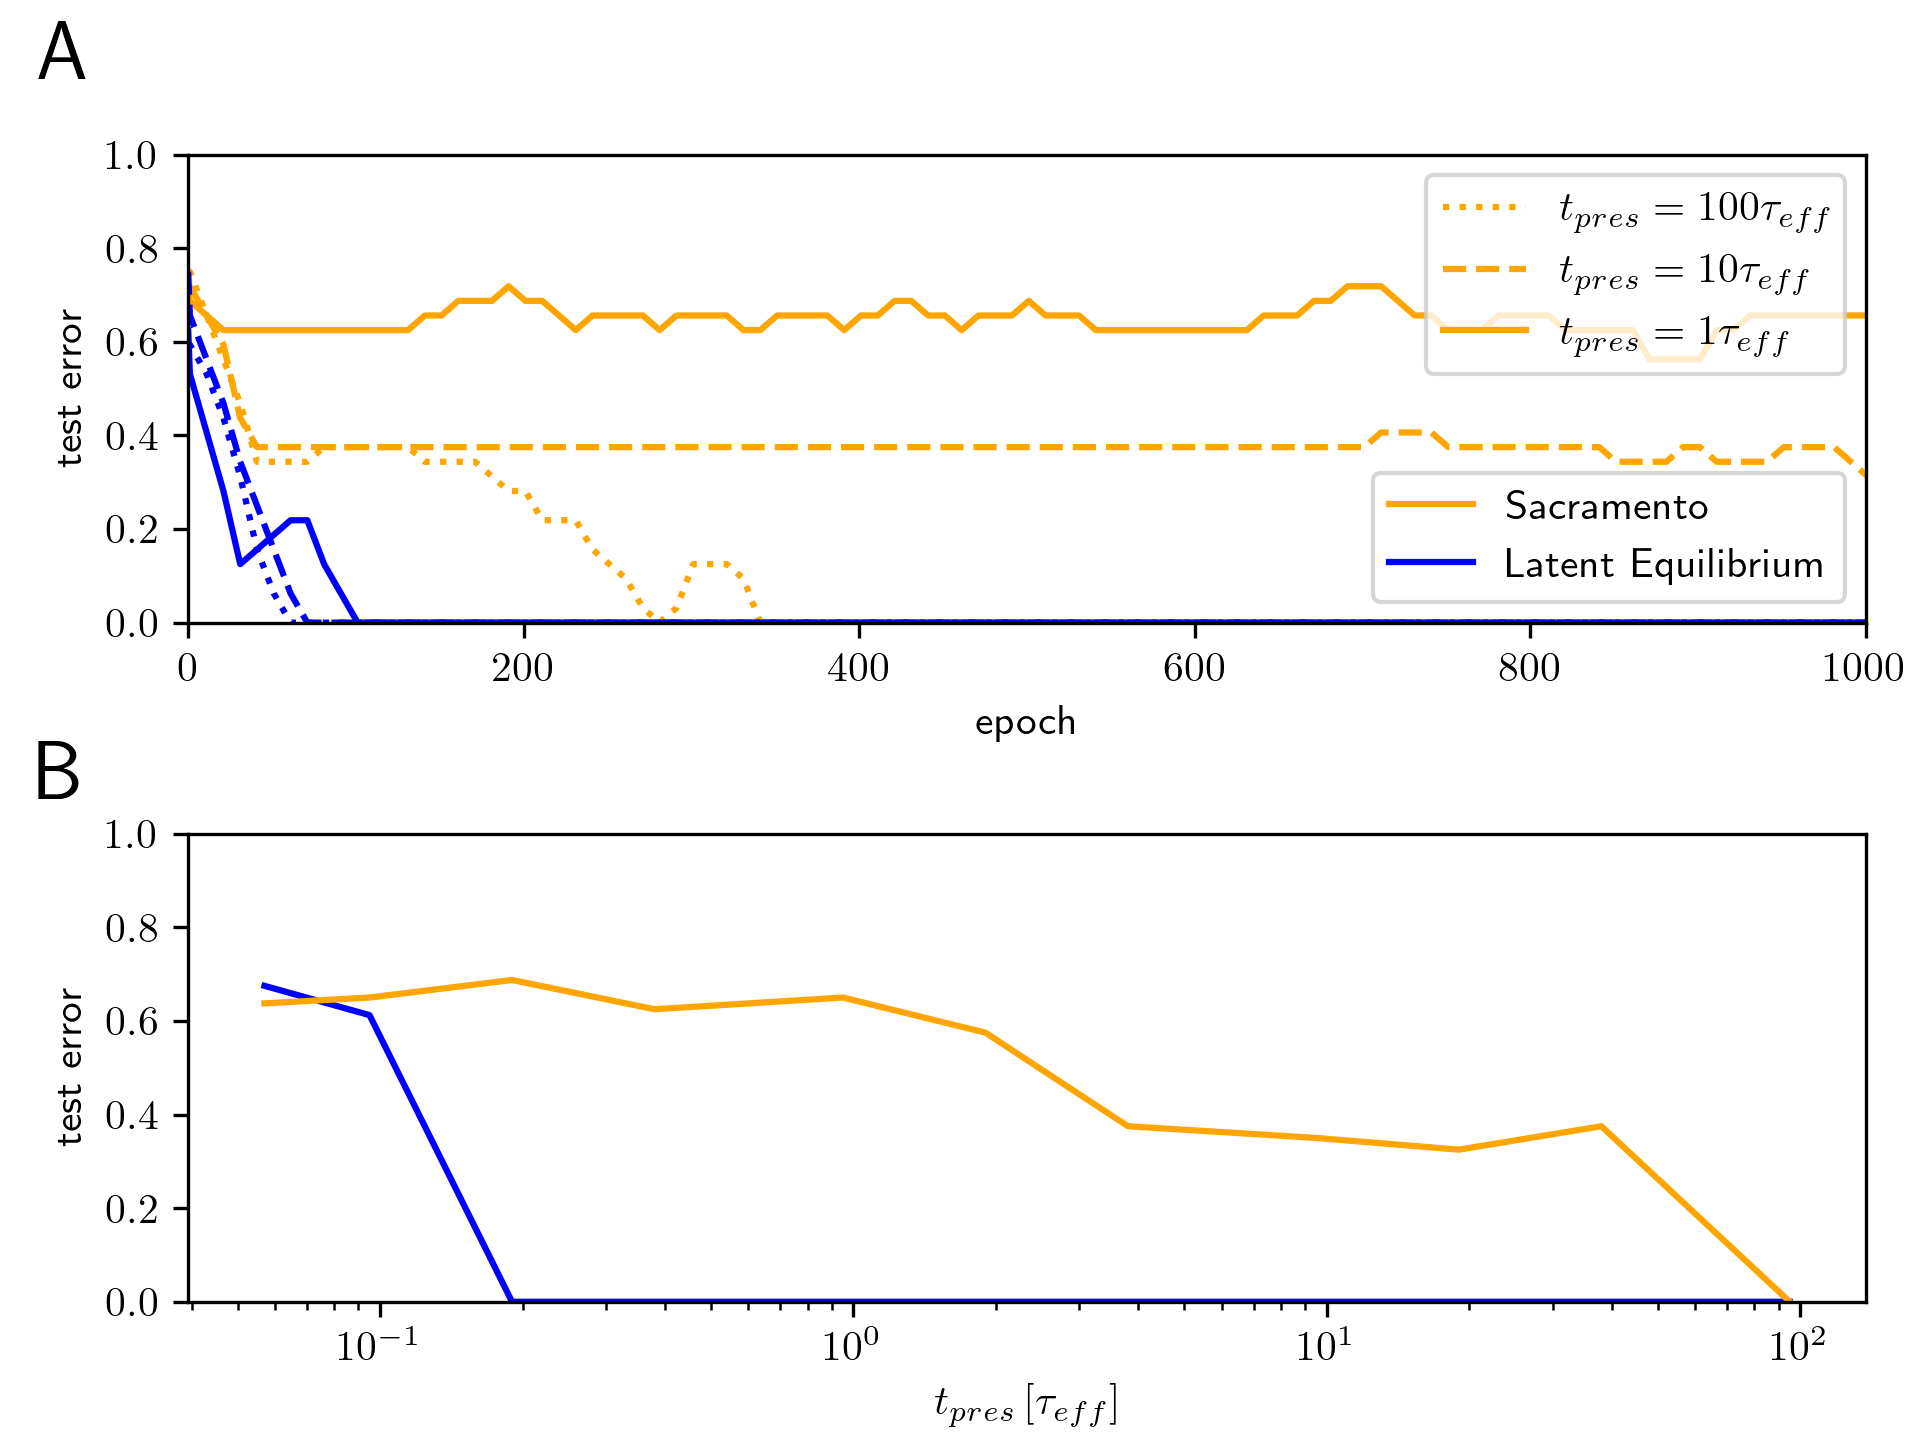
\includegraphics[width=0.9\textwidth]{fig_3_numpy}
    \caption{Replication of Figure \ref{fig-bars-le-snest} using a re-implementation of the \cite{Haider2021} code in
        python. Resulting performance matches the original results exactly, proving that my replication can serve as a
        baseline for comparing the NEST implementation}
    \label{fig-bars-le-numpy}
\end{figure}


\begin{figure}[t]
    \centering
    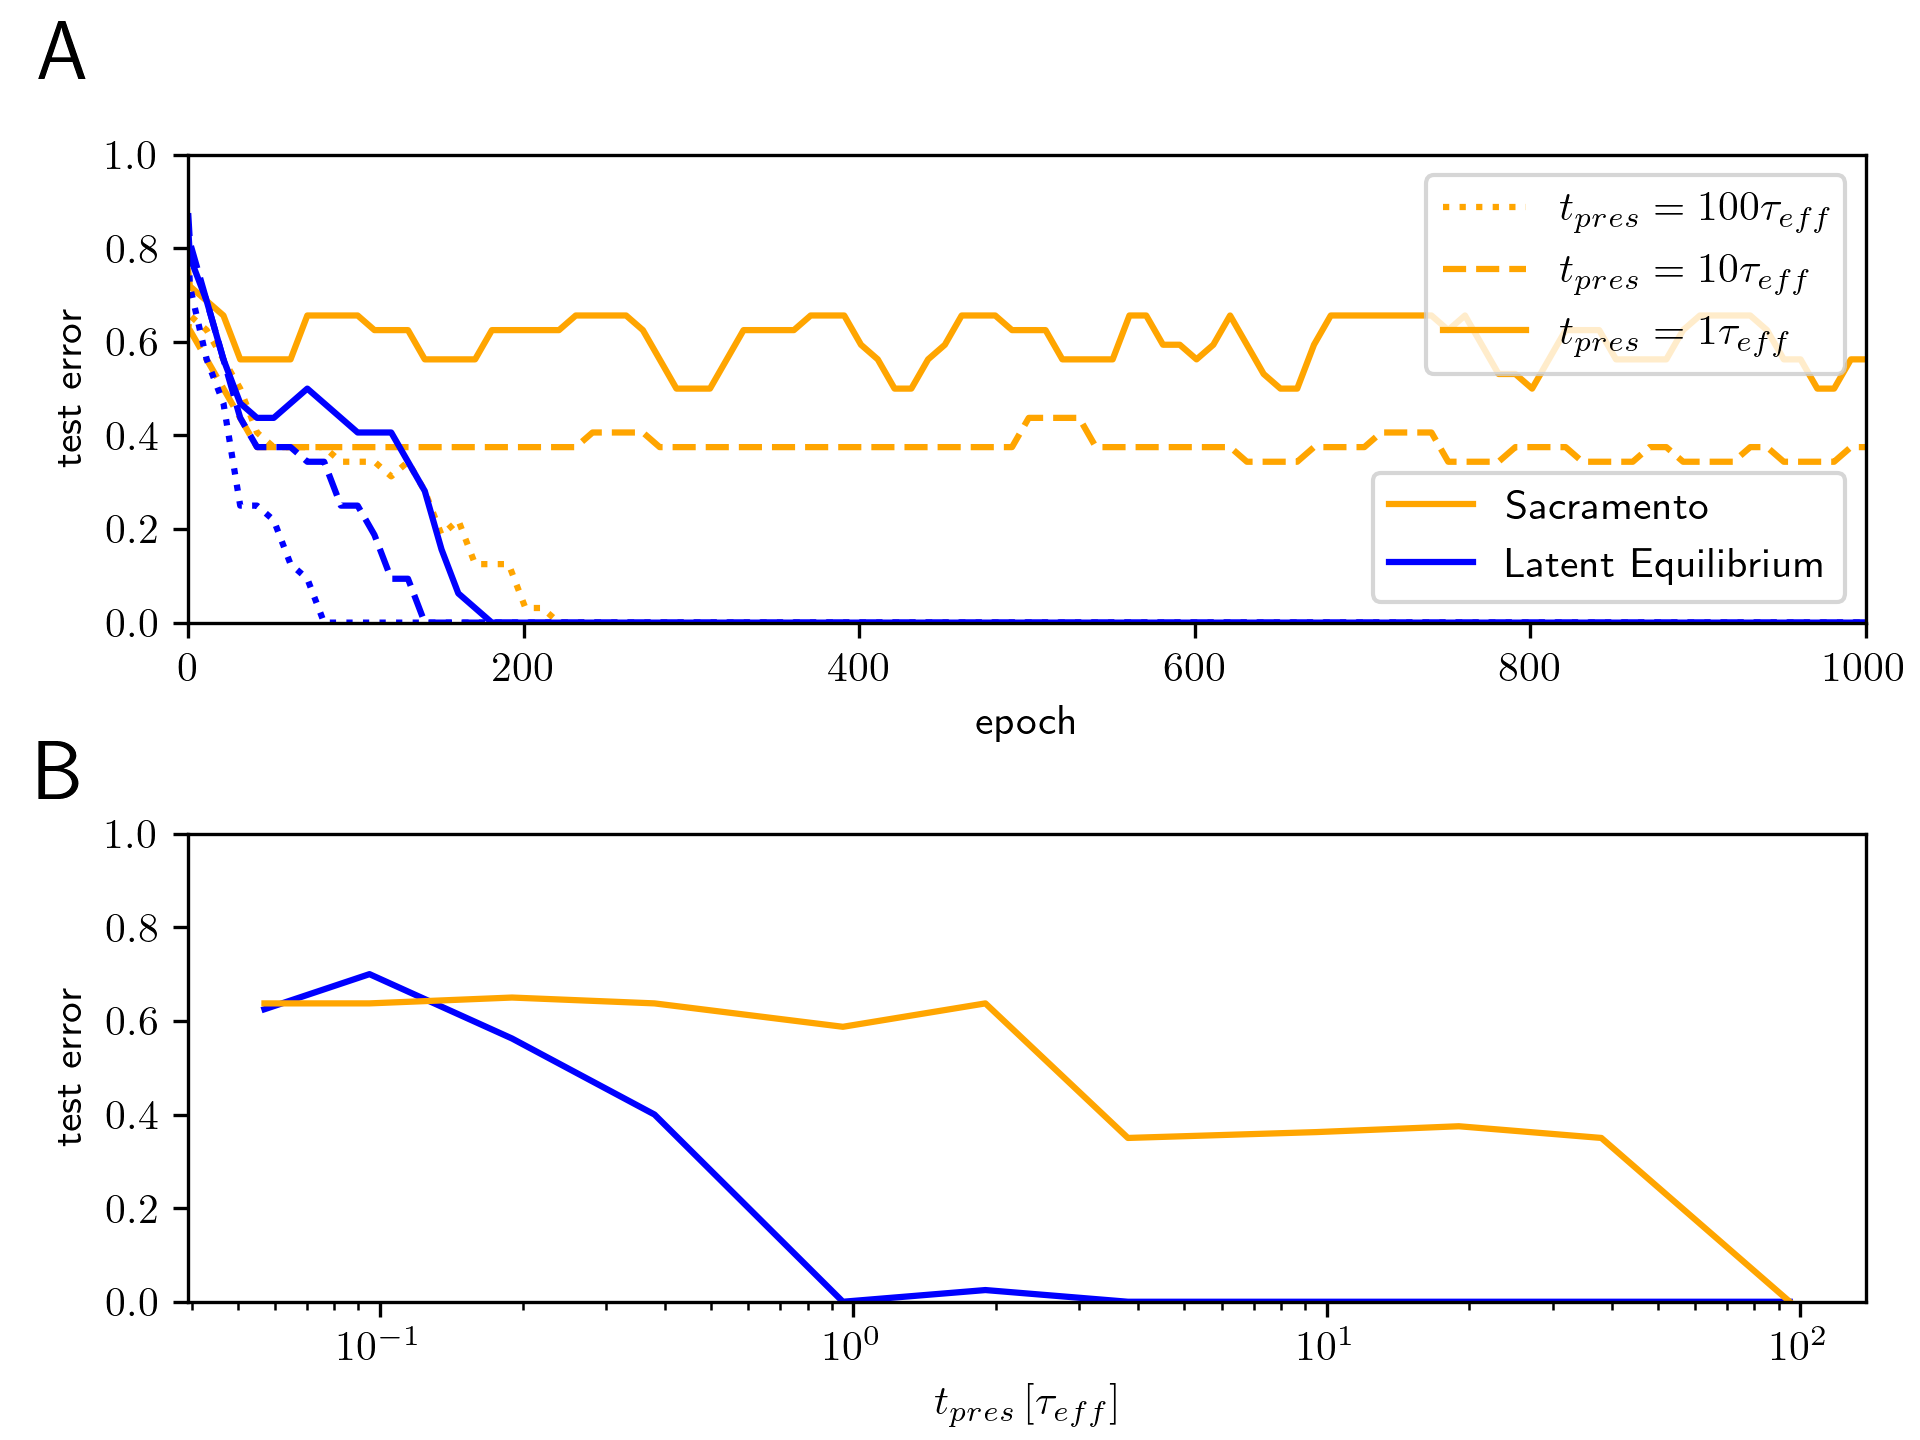
\includegraphics[width=0.9\textwidth]{fig_3_rnest}
    \caption{Replication of Figure \ref{fig-bars-le-snest} using networks of rate neurons in the NEST simulator.}
    \label{fig-bars-le-rnest}
\end{figure}


